\documentclass[12pt, twoside]{article}
\usepackage[francais]{babel}
\usepackage[T1]{fontenc}
\usepackage[latin1]{inputenc}
\usepackage[left=5mm, right=5mm, top=5mm, bottom=5mm]{geometry}
\usepackage{float}
\usepackage{graphicx}
\usepackage{array}
\usepackage{multirow}
\usepackage{amsmath,amssymb,mathrsfs}
\usepackage{textcomp}
\pagestyle{empty}
\usepackage{soul}
\usepackage{eurosym}


\begin{document} 



\begin{flushleft}
NOM PRENOM: \ldots \ldots \ldots \ldots \ldots \ldots \ldots \ldots \ldots
 \end{flushleft}


\begin{center}
{\fbox{$6^{e}8$ \qquad \qquad \textbf{\large{Devoir surveill� 2 }}
\qquad \qquad 15/11/2013}}
\end{center}


\bigskip

\begin{center}

\begin{tabular}{|c|c|c|c|}

 \hline
 
 \quad & un peu & beaucoup & pas du tout \\
\hline

J'ai r�vis� & \quad & \quad  & \quad \\

\hline

J'ai r�ussi & \quad & \quad & \qquad \\

\hline
\end{tabular}
\end{center}


\bigskip

\textit{Les exercices 1, 2, 3 et 4 sont � faire sur la photocopie. Les
autres sont � faire sur votre feuille pr�par�e.}

\bigskip


\ul{\textbf{Exercice 1:}} \textit{(1,5 points)}

\begin{enumerate} 
  \item Tracer en vert le segment joignant les points R et S.
  \item Tracer en rouge la droite passant par les points R et T.
  \item Tracer en bleu la demi-droite d'origine T et passant par S. 
\end{enumerate}

\bigskip

\ul{\textbf{Exercice 2:}} \textit{(2 points)} Relier chaque phrase � sa notation
math�matique.

\begin{center}
\begin{tabular}{lccc}
Le segment d'extr�mit�s M et P \qquad & $\bullet$ \qquad \qquad & \qquad
\qquad $\bullet$ & [PM) \\

\quad \\



La demi-droite passant par P d'origine M \qquad & $\bullet$ \qquad \qquad &
\qquad \qquad $\bullet$ & [MP) \\


\quad \\


La droite passant par les points M et P \qquad & $\bullet$ \qquad \qquad &
\qquad \qquad $\bullet$ & [MP] \\


\quad \\


La demi-droite d'origine P passant par M \qquad & $\bullet$ \qquad \qquad &
\qquad \qquad $\bullet$ & (PM) \\
\end{tabular}
\end{center}

\bigskip

\ul{\textbf{Exercice 3:}} \textit{(2,5 points)} 

\begin{tabular}{cc}
\begin{minipage}{10cm} 


\quad 


Compl�ter par les symboles $\in$
ou $\notin$ :

\quad



$A \ldots \ldots [PI]$ \qquad  \qquad $R$ \ldots \ldots $(AP)$


\quad



$A \ldots \ldots (PI)$ \qquad \qquad $A \ldots \ldots [RH)$

\quad 



\qquad \qquad \qquad  \qquad \qquad $R \ldots \ldots (AR]$
\end{minipage}

&
\begin{minipage}{8cm}
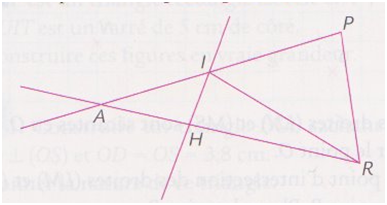
\includegraphics[width=7cm]{images/ex3.png}
\end{minipage}
\end{tabular}


\bigskip

\medskip



\ul{\textbf{Exercice 4:}} \textit{(3 points)} 


\begin{tabular}{cc}
\begin{minipage}{9cm}
\begin{enumerate}
  \item Tracer la droite $(d_1)$ perpendiculaire � la droite $(d)$ passant par
  A.
  \item Tracer la droite $(d_2)$ perpendiculaire � la droite $(d)$ passant par
  B.  
  \item Tracer la droite $(d_3)$ parall�le � la droite $(d)$ passant par
  B.  
\end{enumerate}
\end{minipage}
&
\begin{minipage}{9cm}

\qquad \qquad \quad
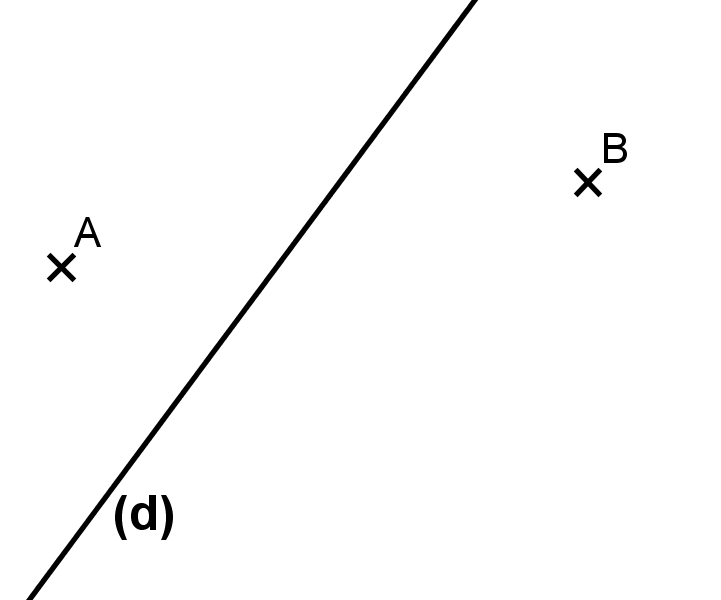
\includegraphics[width=55mm]{images/ex4.png}
\end{minipage}
\end{tabular}


\bigskip

\ul{\textbf{Exercice 5:}} \textit{(4,5 points)}

\enskip

\begin{tabular}{cc}
\begin{minipage}{14cm}
\begin{enumerate}
  \item Que peut-on dire des droites (AD) et (BC)? 
  \item \textbf{Recopier} et compl�ter:
  
  Les droites (AD) et (BC) sont \ldots \ldots parce qu'elles sont toutes les
  deux \ldots \ldots � la droite \ldots \ldots.
  
   
  

\end{enumerate}
\end{minipage}
&
\begin{minipage}{4cm}
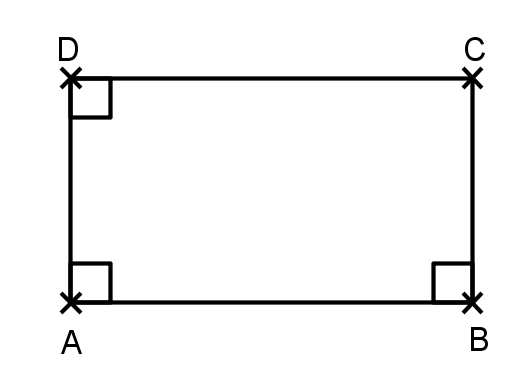
\includegraphics[width=4cm]{images/ex5.png} 
\end{minipage}
\end{tabular}


\begin{enumerate}
  \item [3.] Que peut-on dire des droites (DC) et (BC)?
  \item [4.]
Citer la propri�t� du cours qui permet de l'affirmer.
 
  \item [5.] Quelle est la nature du quadrilat�re ABCD?  
\end{enumerate}


\bigskip

\ul{\textbf{Exercice 6:}} \textit{(3 points)}


\enskip

Les phrases ci-apr�s permettent de donner le programme de construction de la
figure mais elles sont �crites dans le d�sordre.
Remettre ces phrases dans l'ordre.

\enskip


\begin{tabular}{cc}
\begin{minipage}{12cm}
\begin{enumerate}
  \item Tracer la droite perpendiculaire � la droite $(d_1)$ et passant par A;
  elle coupe $(d_1)$ en C.
  \item Placer un point B qui n'appartient ni � la droite $(d_1)$ ni � la
  droite $(d_2)$.
  \item Tracer deux droites $(d_1)$ et $(d_2)$ s�cantes en E.
  \item Tracer la droite parall�le � la droite $(d_1)$ et passant par B; elle
  coupe $(d_2)$ au point A.
\end{enumerate}
\end{minipage}
&
\begin{minipage}{6cm}
\begin{center}
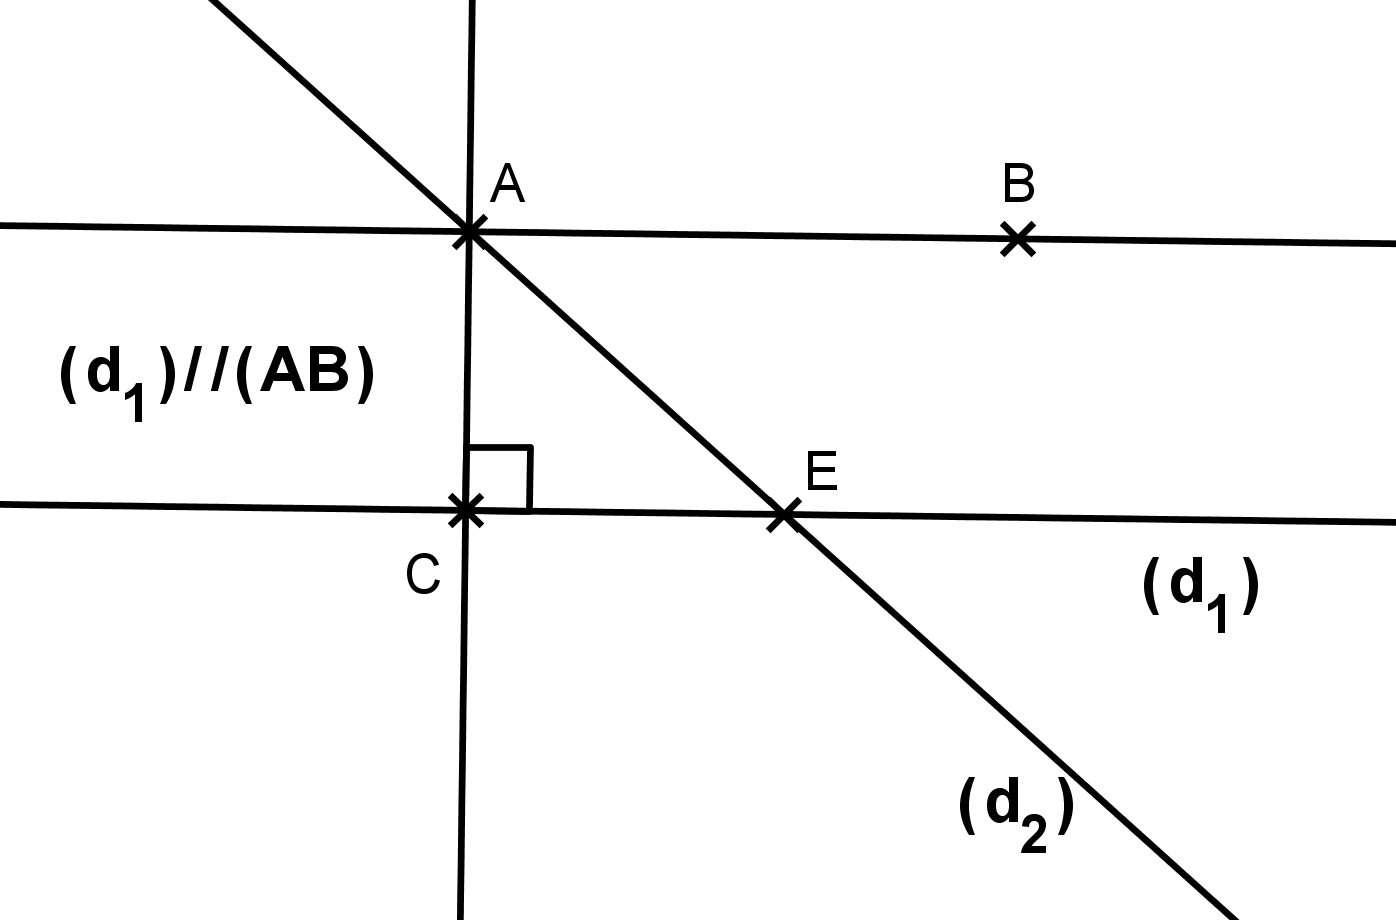
\includegraphics[width=6cm]{images/ex6.png} 
\end{center}
\end{minipage}
\end{tabular}


\bigskip

\ul{\textbf{Exercice 7:}} \textit{(3,5 points)}

\begin{enumerate}
  \item Tracer un triangle ABC.
  \item Placer un point D tel que: $D \in [AB)$ et $D \notin [AB]$.
  \item Placer un point E tel que: $E \in [CA)$ et $E \notin [AC]$.
  \item Placer un point F qui appartient � la droite (DC) et qui est align�
  avec les points E et B.
\end{enumerate}


\bigskip

%\rule{19cm}{0.5pt}

\bigskip

\bigskip

\bigskip

\bigskip

\bigskip

\bigskip

\begin{enumerate}
  \item [3.] Que peut-on dire des droites (DC) et (BC)?
  \item [4.]
Citer la propri�t� du cours qui permet de l'affirmer.
 
  \item [5.] Quelle est la nature du quadrilat�re ABCD?  
\end{enumerate}


\bigskip

\ul{\textbf{Exercice 6:}} \textit{(3 points)}


\enskip

Les phrases ci-apr�s permettent de donner le programme de construction de la
figure mais elles sont �crites dans le d�sordre.
Remettre ces phrases dans l'ordre.

\enskip


\begin{tabular}{cc}
\begin{minipage}{12cm}
\begin{enumerate}
  \item Tracer la droite perpendiculaire � la droite $(d_1)$ et passant par A;
  elle coupe $(d_1)$ en C.
  \item Placer un point B qui n'appartient ni � la droite $(d_1)$ ni � la
  droite $(d_2)$.
  \item Tracer deux droites $(d_1)$ et $(d_2)$ s�cantes en E.
  \item Tracer la droite parall�le � la droite $(d_1)$ et passant par B; elle
  coupe $(d_2)$ au point A.
\end{enumerate}
\end{minipage}
&
\begin{minipage}{6cm}
\begin{center}
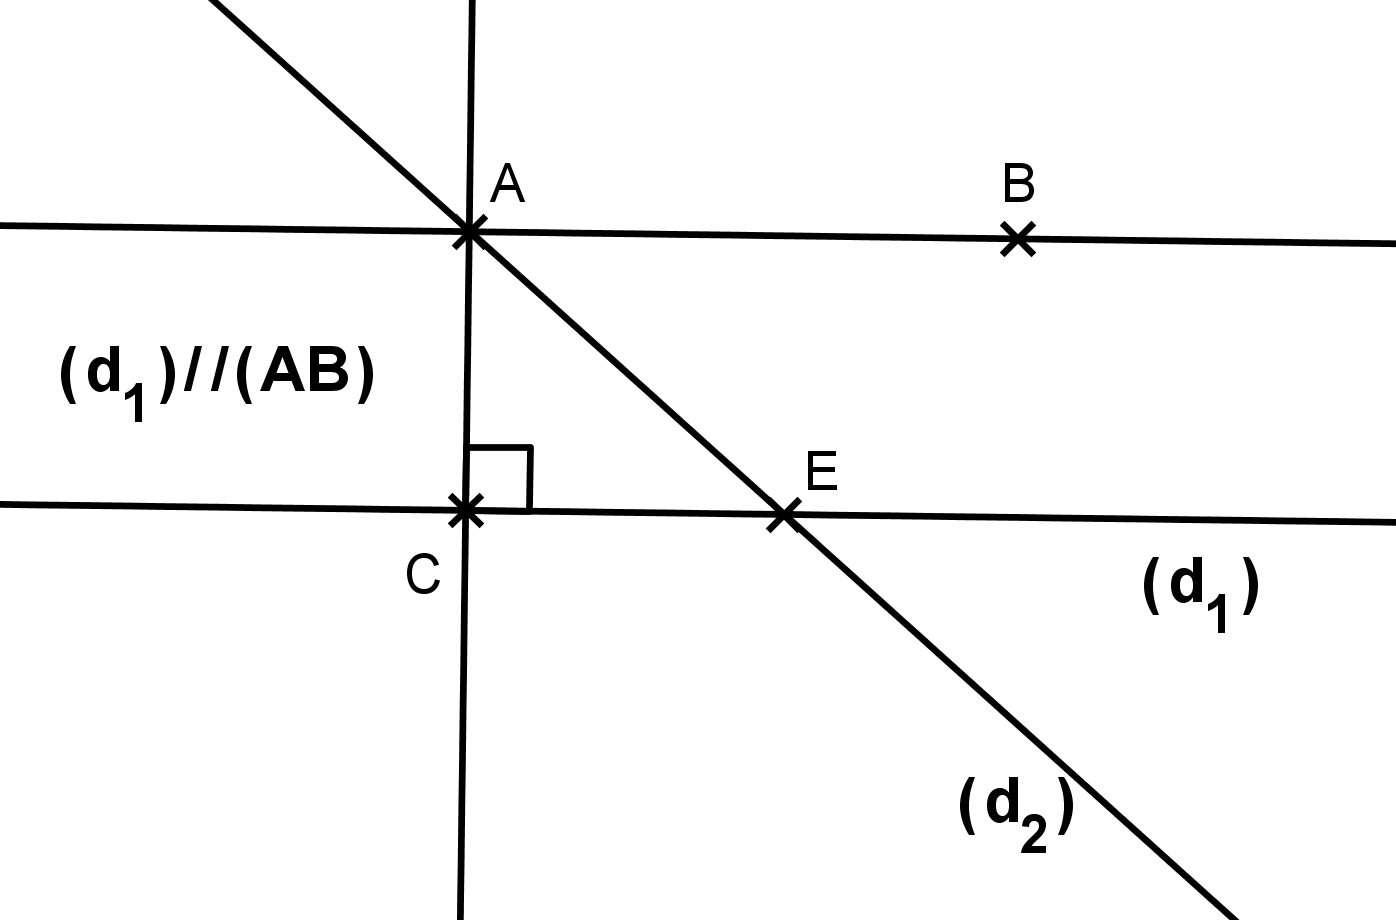
\includegraphics[width=6cm]{images/ex6.png} 
\end{center}
\end{minipage}
\end{tabular}


\bigskip

\ul{\textbf{Exercice 7:}} \textit{(3,5 points)}

\begin{enumerate}
  \item Tracer un triangle ABC.
  \item Placer un point D tel que: $D \in [AB)$ et $D \notin [AB]$.
  \item Placer un point E tel que: $E \in [CA)$ et $E \notin [AC]$.
  \item Placer un point F qui appartient � la droite (DC) et qui est align�
  avec les points E et B.
\end{enumerate}
\end{document}
